\chapter{Support Optimization Algorithm}
\label{cha:support_opt_alg}


\section{Pipeline Overview}
\label{sec:pipeline_overview}

The support structure optimization algorithm we are proposing is organized ino a pipeline
composed of 8 steps, of those the first and last are simple I/O steps (namely Importing and Exporting).
Then the steps two to four (Criticality Detection, Floating Regions Detection and Criticality Grouping)
are simple pre-processing steps that perform some operations in order to prepare data for the following
steps.
Finally steps five to seven (Contact Points Optimization, Contact Points Grouping and Support
Structure Optimization) are the real ``Optimization'' steps, that perform the optimization
of the actual support. This operation is performed in three stages, rather than a single optimization 
process for a more efficient computation, infact we can assume that the decision about where to place
contact points in the areas to support is (roughly) independent from the decision on how to build a
structure that reach those points, this allow to take the decision separately, and have two simpler
problems instead of one complex one. This approach is quite common in literature, infact it has
been used by Zhang et. al. \cite{ZHANG2020117} (the second paper we cited in the previous literature chapter).
The following lists show the steps of the pipeline in order, with a small description of what they do:

\begin{itemize}
    \item \textbf{Importing:} This step load the model and perform some simple re-meshing operations in order
    to reduce the amount of triangles in the mesh in order to obtain better performances.
    \item \textbf{Criticality Detection:} This step detect the critical regions (the points where the
    surface is too steep, and a support is required)
    \item \textbf{Floating Regions Detection:} This step detect the ``Floating regions'' (areas
    of the model that, while being printed are completely detached from the plate for a period of time,
    as the connection is provided by layers above)
    \item \textbf{Criticality Grouping:} This step groups the critical areas detected in the step 2 into
    some areas that can be optimized separately (for more efficient computation)
    \item \textbf{Contact Points Optimization:} This step identify an optimal set of points where
    supports will be placed using a genetic algorithm and a cost function.
    \item \textbf{Contact Points Grouping:} This step group the contact points into areas based on proximity,
    this step is once again performed in order to optimize the different areas separately.
    The optimization is done using a Compositional Pattern Producing Network Based Genetic Algorithm.
    \item \textbf{Support Structure Optimization:} This step optimize the support structure using a genetic
    algorithm, this step is where the stiffness evaluation algorithm we developed previously is used.
    \item \textbf{Exporting:} In the final step we generate a support structure in a mesh based 
    on the optimized parameters, the structure is then exported in STL format.
\end{itemize}


\section{Importing}
\label{sec:importing}

The importing stage is conceptually very simple, A mesh of the object we want to generate support for
is loaded, and then re-meshed.
Re-meshing is a simple procedure that involve starting from a mesh that represent 
a specific object, and then apply a transformation with the aim of obtaining a different
mesh, that represent the same object, using a different set of triangles that satisfy 
some specific properties.
figure \ref{fig:remeshing} show three different meshes that represent the same object,
the first one is minimizing the number of triangles necessary to describe the object,
but is resulting in a set of triangles that is very irregular. The second image show
a re-meshing of the first one, where triangles are divided into smaller and smaller pieces
in order to obtain more regular triangles. The third one is also a re-meshing, but 
it is a more aggressive one, and results in smaller triangles.
For this project we have used an incremental remaster (an algorithm that perform 
recessing by means of progressively splitting and merging triangles in order to obtain
some desired properties). The specific implementation was taken from the popular
rust library ``baby-shark'' \cite{babyshark}.

\begin{figure}[h]
    \centering
    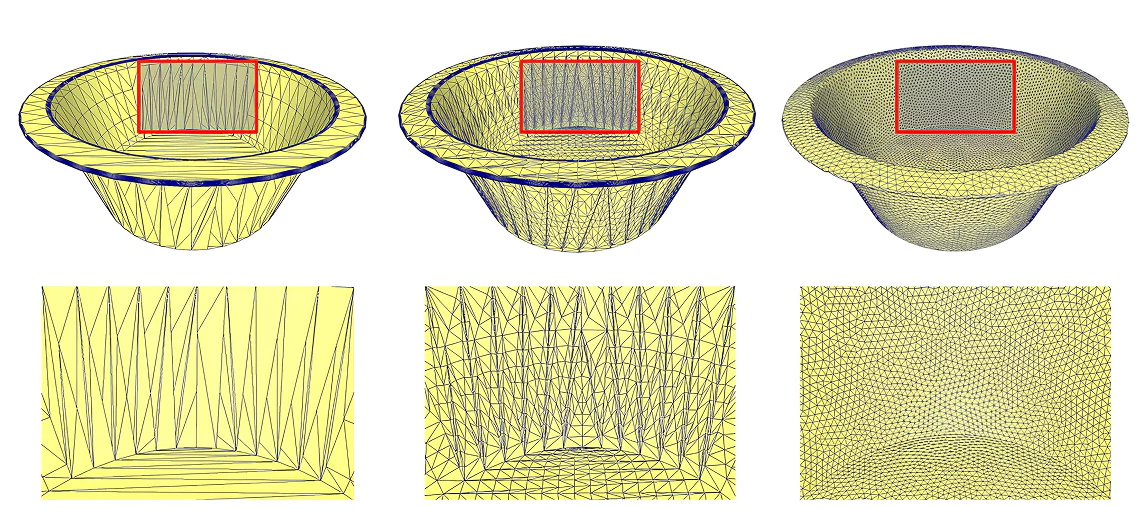
\includegraphics[width=0.5\textwidth]{images/remeshing.png}
    \caption{Example of a re-meshing operation (source: \cite{remeshing})}
    \label{fig:remeshing}
\end{figure}

There are two reasons why re-meshing is applied as part of the loading stage.
The first one is purely a performance reason, infact in order to generate support structure
we don't need an high definition mesh, instead a good approximation is enough. For this reason
the re-meshing process target an edge length in the range of 0.3 - 1.0 mm. this provide a sufficient
level of accuracy while also resulting in a manageable number of triangles, even for large meshes,
which helps the algorithm's performance.
The second reason why re-meshing is important has to do with the representation of the mesh
in the algorithm, infact the last step of the loading procedure is converting 
the mesh into a set graph, where every triangle is a node, and each node is connected
to three other neighbors (one for each side of the triangle.)
Generally speaking we would want all triangle to be as close to an equilateral as possible,
in such a way every connection inside the graph would have ruffly the same length; This
fact is a precondition necessary for the correct functioning of the next stages in the pipeline.
The re-meshing algorithm is therefore also used to ensure triangles have ruffly the same size,
and are ruffly equilateral.

\section{Criticality Detection}
\label{sec:crit_detection}

The first step in the generation of automatic support is of course knowing what zones must be supported.
Generally speaking the presence of a support or not is usually achieved with a simple check of the 
overhanging angle (as we already in the introduction \ref{sec:role_of_sup}).
One of the most basic technique for criticality detection is to simply take angle formed by the 
surface normal of a triangle, and a vector facing downward, and compare that to the threshold of what
is consider acceptable, in order to detect the critical areas.
Most 3D printing software use methods derived the one we just described with a few refinement
key refinements such as for example bridge detection, detection of areas that are ``floating''
etcetera. Our method also inspired by that basic idea, but is slightly different from the 
methods currently used in most commercial 3D printing software, as it's built with a different 
paradigm. Instead of simply detecting a simple boolean value that tell if a surface is critical
or not, our method aim to provide a cost function that, if minimized, reduces the amount of critical
areas there are in a specific model. The reason why this approach was chosen is straightforward, as 
is a simple consequence of the fact that we will need a cost function in order to apply a genetic-algorithms
based optimizer in the following steps.

Now that we explained the reasoning behind the creation of a custom solution for criticality detection
we can begin explaining our implementation. Algorithm \cref{alg:crit_det} show the pseudo-code of 
our implementation of a criticality detection procedure.
The key idea behind our solution is to assign to every node in the mesh graph a ``criticality''.
then the critical node are the one that have a criticality different than zero. This model has the benefit
that it can be easily transformed into a cost function by summing all the criticality score and 
weighting them by the area of the triangle they are associated to.
The second key idea that our solution brings to the table is the concept of ``criticality propagation''
This concept represent the fact that criticality is not an arbitrary value assigned to every single
triangle, regardless of the neighbors, instead the criticality is ``propagated'' from the bottom to the
top. This means that criticality increases every time the object have an overhanging angle that is too hig,
and decreases every time the criticality angle is too low. This is important because otherwise, a single
triangle inside the mesh with a sufficiently low overhanging angle would make an entire zone
less critical, or in the same way a single support could singlehandedly make a large critical area
no longer critical. Figure \ref{fig:critical_detect} show a mesh of a dragon, with the green areas
being the meshes with a criticality score of zero, while the red areas are the critical one.
In here we can see the effect that criticality propagation has on the structures.
in the bottom part of the dragon's wing we can see that the critical area is quite large,
even tho, the overhanging angle is quite small. We can get a sense on why propagation is important
by looking at figure \ref{fig:critical_detect_no_prop} and \ref{fig:critical_detect}.
In the former we see what are the critical regions if no propagation is applied, mean while in the second one
we see the same output, but propagation are applied. Te most notable difference is in the bottom part
of the dragon's wing, as we can see, in the version with no propagation there is a tiny critical area
in the tip of the wing, but as soon as the overhanging angle is small enough, the critical are disappear.
In contrast in the version that has propagation the criticality start at an high value in the top bottom
part of the wing, and require a bit of time for the score to reach zero, resulting in a much larger critical
region. This behavior is desirable, as is unreasonable to think that a single support in the tip of the wing
is enough to support the entire area, meaning that criticality propagation play a key role in detecting
more realistic critical regions when some part of the model are ``floating''.


\begin{figure}[h]
    \centering
    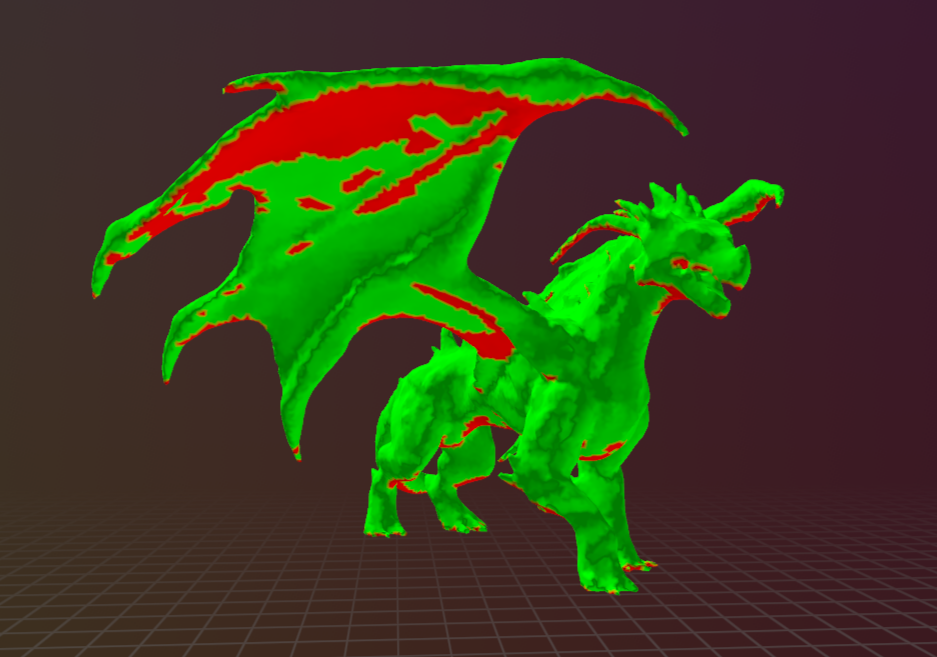
\includegraphics[width=0.5\textwidth]{images/critical_regions_w_no_prop.png}
    \caption{Critical regions detected by our algorithm, if no propagation is used}
    \label{fig:critical_detect_no_prop}
\end{figure}

\begin{figure}[h]
    \centering
    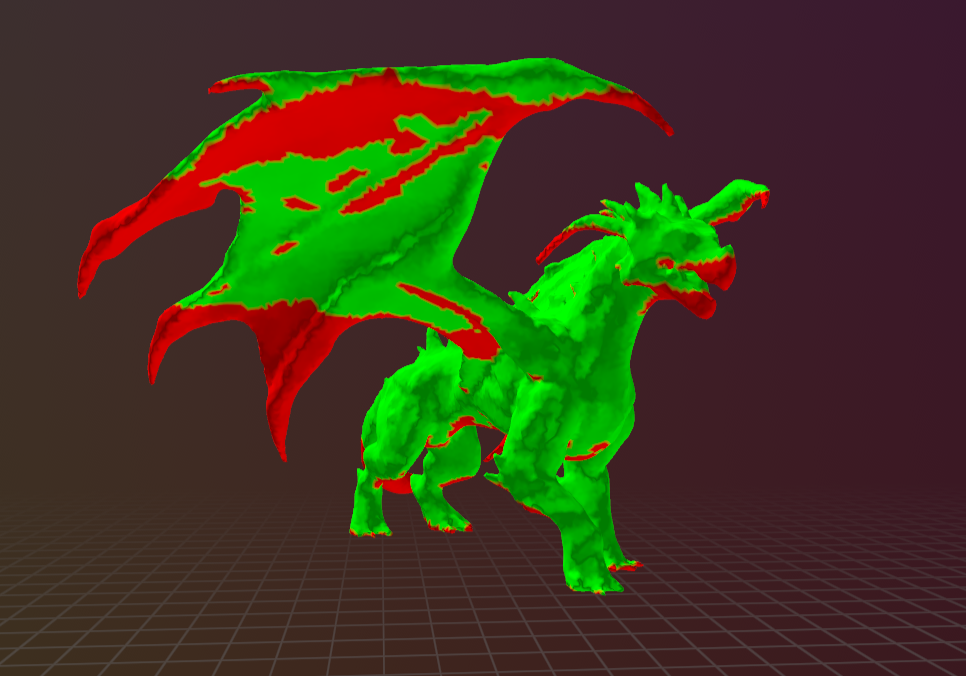
\includegraphics[width=0.5\textwidth]{images/critical_regions.png}
    \caption{Critical regions detected by our algorithm}
    \label{fig:critical_detect}
\end{figure}



\begin{algorithm}[H]
\caption{Criticality Detection}
\begin{algorithmic}[1]
    \Require $G$ Graph that represent the mesh
    \Ensure $C$ Dictionary that associate a cost for every node in the graph

    \Procedure{LayerOf}{$n$} \Comment{Calculate the layer of node $n$}
        \State \Return $\left\lfloor{\frac{\Call{Height}{n}}{L_{height}}}\right\rfloor$
    \EndProcedure

    \Statex

    \Procedure{PropagationCost}{$G, f, t$} \Comment{Calculate propacation factor of the link $f$(rom) $t$(o)}
        \State $\varphi \gets \Call{AngleBetween}{f, t}$ \Comment{We start from the angle between the two nodes}
        \State $\varphi' \gets \varphi - \varPhi_t$ \Comment{We compared to the threshold, as small gradients are OK}
        \State $\varphi'' \gets \Call{Clamp}{\varphi', \varPhi_{lb}, \varPhi_{ub}}$ \Comment{We clamp it, to avoid too high propagation factor}
        \State $d \gets \Call{Distance}{f, t}$ \Comment{Distance factor (long distance are more critical than short one)}
        \State \Return $K_{prop} \cdot d \cdot \varphi''$
    \EndProcedure

    \Statex

    \Procedure{CriticalityOf}{$G, n, \mathcal{M}$}
        \If {$\Call{Height}{n} = 0$} \Comment{Nodes to the ground are never critical}
            \State \Return 0
        \EndIf
        \State $c \gets $ CRITICALITY\_MAX \Comment{Initialize criticality at max value}
        \For{$a \in \Call{AdjacentNodes}{G, n$}} \Comment{Iterate over adjacent nodes}
            \If {$\Call{LayerOf} {a} <= \Call{LayerOf}{n} \land a \in M$}
                \State $c_a \gets M(a) + \Call{PropagationCost}{a, n}$
                \State $c \gets \Call{Min}{c, c_a}$
            \EndIf
        \EndFor
        \State \Return $\Call{Max}{c, 0}$ \Comment{Criticality is always greater of equal than zero}
    \EndProcedure

    \Statex

    \Procedure{PropagateInLayer}{$G, l, \mathcal{M}$}
        \State $ PriorityQueue \gets \emptyset$
        \For{$n$ in $l$} \Comment{Initialize the priority queue with the cost propageted by the laeyer below}
            \State $c \gets \Call{CriticalityOf}{G, n, \mathcal{M}}$
            \State $\Call{Push}{PriorityQueue, n, c}$
        \EndFor
        \While {$\lnot \Call{Empty}{PriorityQueue}$}
            \State $n, c = \Call{Pop}{PriorityQueue}$ \Comment{Extract node with the lowest criticality}
            \State $\mathcal{M}(n) \gets c$ \Comment{Mark the criticality in the memory}
            \For{$a$ in \Call{Adjacent}{$G, n$}} \Comment{Neighbors might now have lower criticality, update them}
                \State $c \gets \Call{CriticalityOf}{G, a, \mathcal{M}}$
                \State $\Call{TryUpdatePriority}{PriorityQueue, a, c}$
            \EndFor
        \EndWhile
        \State \Return $0$;
    \EndProcedure
    
    \Statex

    \Procedure{CriticalityDetection}{$G$}
        \State $C \gets \emptyset$

        \For{l in \Call{Layers}{$G$}}
            \State \Call{PropagateInLayer}{$G, l, C$} \Comment{Propaget the cost one layer at a time}
        \EndFor

        \State \Return $C$
    \EndProcedure
\label{alg:crit_det}
\end{algorithmic}
\end{algorithm}


\subsection{Algorithm Overview}
To explain \cref{alg:crit_det} we must start from the concept of layer.
Eery node in a graph is assigned to a layer (represented by an integer value),
the ``LayerOf'' function simply associate a node with is layer, and is simply using
the node's height as the discrimination factor;
The reason why layers are important is that the criticality can be propagated only from
elements of the same layer, or layer below, it can't go below a layer.
The function ``PropagationCost'' take as input two nodes, and calculate the cost that 
is propagated from one to the other in a specific direction, this means that if
node $A$ has criticality $c_a$ and the propagation cost from node $A$ to node $B$ is
$c_{ab}$ than the cost at node $B$ will be upper bounded by he value $c_a + c_{ab}$.
This is an upper bound because it can always be lower if node $B$ has another neighbor
from which it can propagate a lower cost.
It should be noted that this function can return a negative value, this is the case when 
the angle between the two nodes is below the threshold of the maximum overhanging angle, 
and therefore the criticality should decrease.
The function ``CriticalityOf'' is used to calculate the criticality of a node, starting
from nodes that are close to it; In the function we can see how if the node is close to the
ground the criticality is zero (this is obvious, as if a node is attached to the plate it does
not need any support), otherwise the criticality is initialized to the maximum possible value,
and then is reduced if a path is found to propagate a lower criticality value from a neighbor.
The neighbor in order to be eligible must be part of a layer that is the same or lower as the node
currently being evaluated.
Now that we have explained the few ``utility'' functions we can tackle the core part of the algorithm,
this is composed of the two functions ``PropagateInLayer'' and ``CriticalityDetection''.
the idea is that the criticality is propagated from bottom to top, then odes in the graph are organized
in layers, and layers are evaluated from the lowest to the hightest.
The process of evaluating a layer is essential a one pass of a Dijkstra algorithm, where nodes
are explored form the one with the lowest criticality value to the one with the highest.
This process ensure low time complexity while ensuring that every node has the correct criticality value.

\section{Floating Regions Detection}
\label{sec:floating_regions_detection}

Another important pre-processing step is the detection of ``Floating Regions''
As we mentioned in the introduction, a floating region is defined a part of the structure that that while being printed,
is not fully connected to the build plate if not for supports. For example
figure \ref{fig:floating_regions} show the floating regions of the mesh ``Dragon''
highlighted in different colors, while the plain mesh white.
In this section we will not explain why detecting floating regions is necessary,
as that topic will be extensively covered in one of the next sections (specifically \ref{sec:sup_struct_opt_cf}).


\begin{figure}[h]
    \centering
    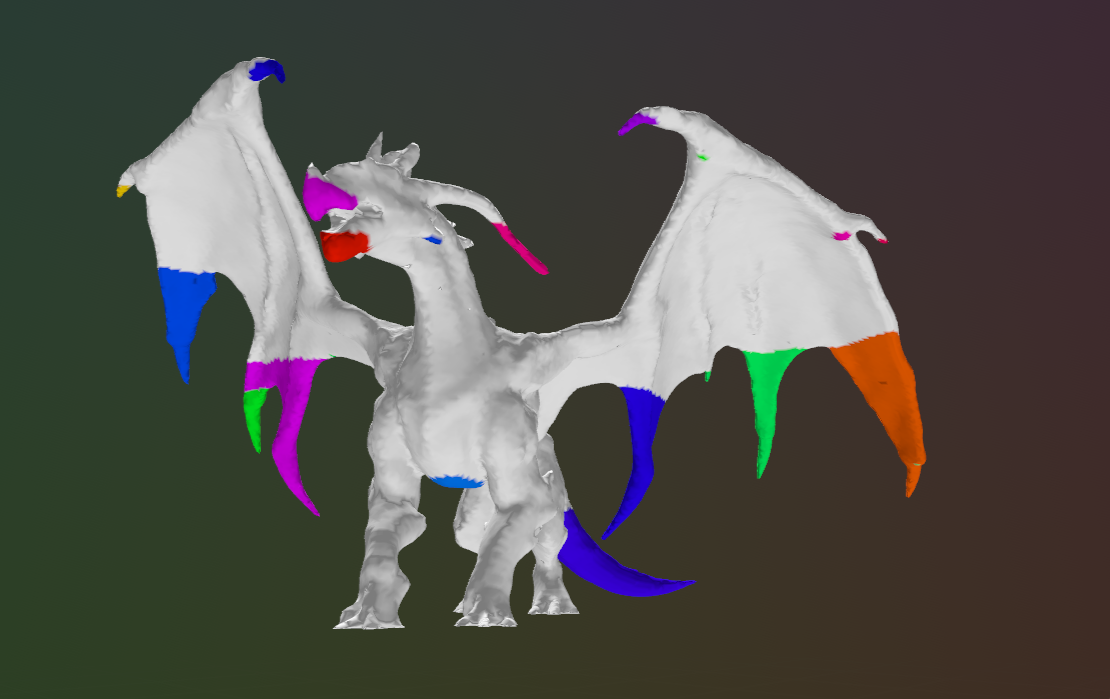
\includegraphics[width=0.5\textwidth]{images/floating_regions_detect.png}
    \caption{Detected floating regions for the test-mesh ``Dragon''}
    \label{fig:floating_regions}
\end{figure}

Efficient detection of floating regions can be achieved using algorithm \cref{alg:float_det}
the idea is that the nodes are sorted from the lowest to the highest, then they are sampled one by one,
and, then visiting the all the nodes reachable form the point, where an arch that go from $A$ to $B$ is 
considered valid only if the layer of $B$ is grater or equal to the layer of $A$.
This ensures that we cannot go ``downward'' when exploring the graph, and therefore that
we cannot explore a floating region unless we start from a point inside that floating region.
While the graph is being explored, we mark nodes that have been visited to avoid visiting the same
node twice, and increasing the time complexity. Once an exploration is completed we can decide if
the explored area is a floating region or not. This can be simply done by checking if the height
of the ``source'' node is equal to zero (or at least is below a certain threshold),
if this is the case we can say that the source was attached to the ground, and therefore
the region is not floating. If this is not the case however, the area we have explored must be a 
floating region. We can also be sure that the nodes we have extracted is the lowest point in the region,
thanks to the sorting we did at the beginning. The sorting also ensures that we start exploring from
the nodes that are close to the ground, avoiding a situation where a floating region is expanded
too much and reach zones that are actually not considered ``floating''.

\begin{algorithm}[h]
\caption{Floating Regions Detection}
\begin{algorithmic}[1]
    \Require $G$ Graph that represent the mesh
    \Ensure $\mathcal{F}$ Set of floating regions 

    \Procedure{ExploreUpward}{$G, s, V$} \Comment{Collect the component reachable going up from $s$}
        \State $R \gets \emptyset$
        \State $Q \gets \{s\}$ \Comment{Initialize the queue with the node}
        \While{$\lnot \Call{IsEmpty}{Q}$} \Comment{repeat untill queue is empty}
            \State $n \gets \Call{Pop}{Q}$
            \State $V(n) \gets true$
            \State $R \gets \Call{Append}{R, n}$
            \For{$a \in \Call{Adjacent}{G, n}$ with } \Comment{Explore adjacent neighbors}
                \If{ $\Call{LayerOf}{a} \geq \Call{LayerOf}{n} \land \lnot V(a)$ } \Comment{Filter by non visited, and $\geq$ layer}
                    \State \Call{Push}{Q, a}
                \EndIf
            \EndFor
        \EndWhile
        \State \Return $R$
    \EndProcedure

    \Statex


    \Procedure{FloatingRegionsDetection}{$G$}
        \State $\mathcal{F} \gets \emptyset, \quad V \gets \emptyset$ \Comment{Detected regions and visited nodes}
        \For{$n \in \Call{SortNodesByHeight}{G}$}
            \If{$V(n)$}
                \State \textbf{continue} \Comment{Already part of a component}
            \EndIf
            \State $R \gets \Call{ExploreUpward}{G, s, V}$ \Comment{Exploring grpah, while only moving ``uppward''}
            \If{$\Call{HeightOf}{s} > 0$} \Comment{If the node is detached from the ground}
                \State $F \gets \Call{AddFloatingRegion}{F, R}$ \Comment{Mark the explored node as a floating region}
            \EndIf
        \EndFor
        \State \Return $\mathcal{F}$
    \EndProcedure
\label{alg:float_det}
\end{algorithmic}
\end{algorithm}



\section{Criticality Grouping}
\label{sec:criticality_grouping}


\section{Contact Points Optimization}
\label{sec:contact_points_opt}


\section{Contact Points Grouping}
\label{sec:contact_points_grouping}


\section{Support Structure Optimization}
\label{sec:sup_struct_opt}

\subsection{Cost Function}
\label{sec:sup_struct_opt_cf}



\section{Exporting}
\label{sec:exporting}
exp


